\documentclass[10pt]{article}
\usepackage{longtable}
\usepackage{float}
\usepackage{wrapfig}
\usepackage{rotating}
\usepackage[normalem]{ulem}
\usepackage{amsmath}
\usepackage{textcomp}
\usepackage{marvosym}
\usepackage{wasysym}
\usepackage{amssymb}
\usepackage{hyperref}
\usepackage{color,soul} % for highlighting
\usepackage{graphicx}
\graphicspath{{/Users/benjaminbass/seacloud/class/earthMaterials/picBank/}}

\usepackage{frame,color}
\usepackage{framed}
\usepackage{minibox}

% \usepackage[T1]{fontenc}
% \usepackage{tilting} %bring title up
% \setlength{\droptitle}{-10cm}

\usepackage[version=3]{mhchem}
% How to Use MChem
% \ce{SO4^2-}
% \ce{^{227}_{90}Th+}
% \ce{A\bond{-}B\bond{=}C\bond{#}D}
% \ce{CO2 + C -> 2CO}
% \ce{SO4^2- + Ba^2+ -> BaSO4 v}


\author{Benjamin Bass}
\date{2 March 2016}
\title{\vspace{-2.0cm}Enstatite} %bring title up temporary Fix

\begin{document}

\maketitle

% \framebox{Use frameboxes until figure out alignmen}

\begin{center}
  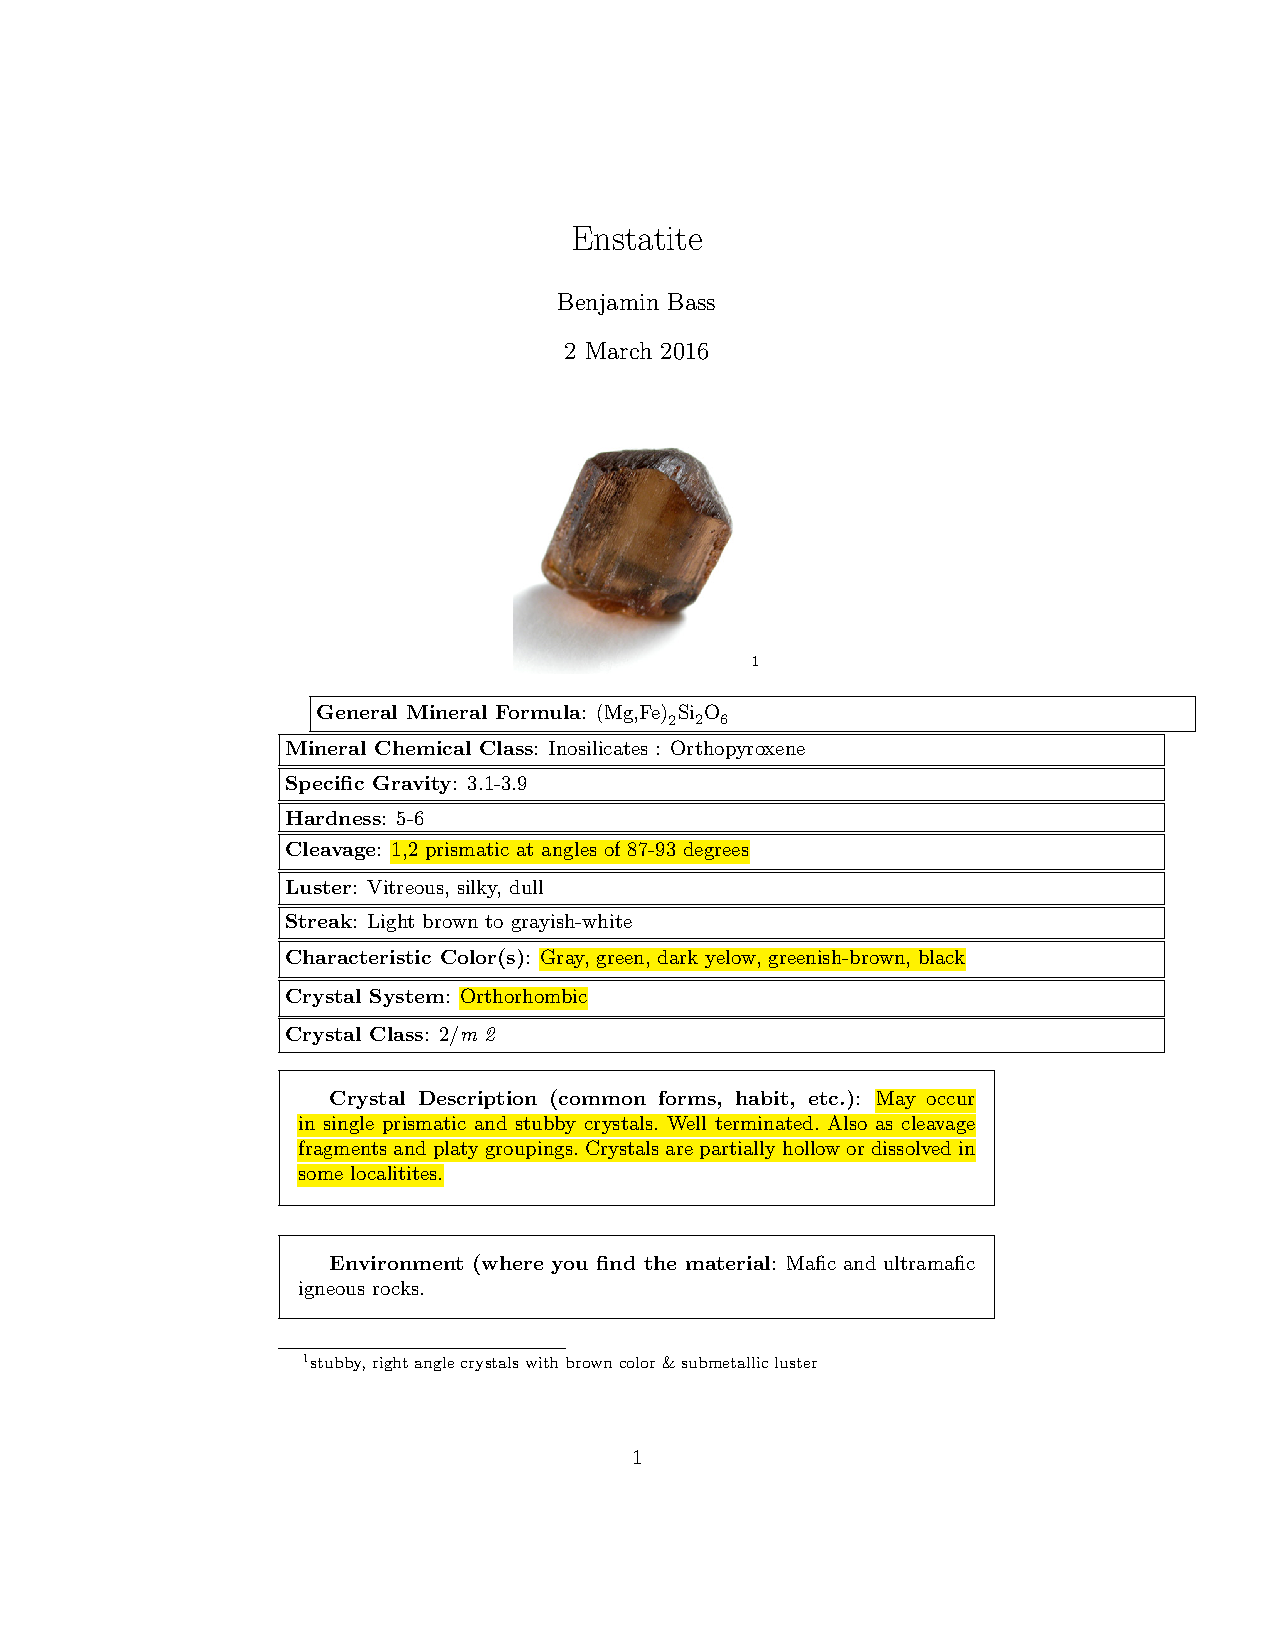
\includegraphics[scale=.40]{enstatite}\footnote{stubby, right angle crystals with brown color \& submetallic luster}
\end{center}



\framebox[15cm][l]{\textbf{General Mineral Formula}: \ce{(Mg\text{,}Fe)2Si2O6} }\
\framebox[15cm][l]{\textbf{Mineral Chemical Class}: Inosilicates : Orthopyroxene }\
\framebox[15cm][l]{\textbf{Specific Gravity}: 3.1-3.9}\
\framebox[15cm][l]{\textbf{Hardness}: 5-6}\
\framebox[15cm][l]{\textbf{Cleavage}: \hl{1,2 prismatic at angles of 87-93 degrees} }\
\framebox[15cm][l]{\textbf{Luster}: Vitreous, silky, dull}\
\framebox[15cm][l]{\textbf{Streak}:  Light brown to grayish-white}\
\framebox[15cm][l]{\textbf{Characteristic Color(s)}:  \hl{Gray, green, dark yelow, greenish-brown, black}}\
\framebox[15cm][l]{\textbf{Crystal System}:  \hl{Orthorhombic}}\
\framebox[15cm][l]{\textbf{Crystal Class}:  2/\it{m} 2}\

\begin{framed}
  \textbf{Crystal Description (common forms, habit, etc.)}: \hl{May occur in single prismatic and stubby crystals. Well terminated. Also as cleavage fragments and platy groupings. Crystals are partially hollow or dissolved in some localitites.}
\end{framed}

\begin{framed}
  \textbf{Environment (where you find the material}: Mafic and ultramafic igneous rocks.
\end{framed}

\begin{framed}
  \textbf{Common Mineral Associations (in samples, also consult text, notes}: Feldspars, Ca-clinopyroxene, hornblende, biotite, garnet.
\end{framed}

\begin{framed}
  \textbf{Scientific Usage/Significance}: None
\end{framed}

\begin{framed}
  \textbf{Industrial or Social Use/Significance}:  Dimension stone/ minor gemstone.
\end{framed}

\begin{framed}
  \textbf{Environmental Significance}: None
\end{framed}

% Possible other Solutions
% \framebox(300,20){\minibox{\textbf{R-Sq}:For example}}

\end{document}
%%% Local Variables:
%%% mode: latex
%%% TeX-master: t
%%% End: